\chapter{Lec 11 - 12 - Optimization}

\section{Optimization for Neural Networks}
Optimization algorithms used for training of deep models differ from traditional optimization algorithms in several ways. In most machine learning scenarios, we care about some performance measure
$P$, that is defined with respect to the test set and may also be intractable. We therefore optimize $P$ only \textbf{indirectly}. We reduce a different cost function $J(\theta)$ in the hope that doing so will improve $P$.\newline\newline
The goal of a machine learning algorithm is to reduce the expected generalization error:
\[J^*(\theta) = E_{(\textbf{x}, y) \sim p_{data}} L(f(\textbf{x}; \theta), y)\]
This quantity is known as the \textbf{risk}. If we knew the true distribution
$p_{data}(\textbf{x}, y)$, risk minimization would be an optimization task solvable by an optimization algorithm. However, when we do not know $p_{data}(\textbf{x}, y)$ but only have a training set of samples, we have a machine learning problem. The simplest way to convert a machine learning problem back into an optimization problem is to minimize the expected loss on the training set. This means replacing the true distribution $p(\textbf{x}, y)$ with the empirical distribution $\hat{p}(\textbf{x}, y)$ defined by the training set. We now minimize the \textbf{empirical risk}:
\[E_{(\textbf{x}, y) \sim \hat{p}_{data}} L(f(\textbf{x}; \theta), y) = \frac{1}{m}\sum_{i=1}^m L(f(\textbf{x}^{(i)}; \theta), y^{(i)})\]
where $m$ is the number of training examples. We optimize the empirical risk, and hope that the risk decreases significantly as well \footnote{A variety of theoretical results establish conditions under which the true risk can be expected to decrease by various amounts}. However, empirical risk minimization is prone to overfitting. Models with high capacity can simply memorize the training set. Furthermore, the most effective modern optimization algorithms are based on gradient descent, but many useful loss functions, such as 0-1 loss, have no useful derivatives.

\subsection{Surrogate Loss}
Sometimes, the loss function we actually care about (e.g. classification error) is not one that can be optimized efficiently. For example, exactly minimizing expected 0-1 loss is typically intractable (exponential in the input dimension), even for a linear classifier. In such situations, one typically optimizes a surrogate loss function instead, which acts as a proxy, but has advantages. For example, the negative log-likelihood of the correct class is typically used as a surrogate for the 0-1 loss.\newline\newline
A very important difference between optimization in general and optimization
as we use it for training algorithms is that training algorithms do not usually halt at a local minimum. A machine learning algorithm usually minimizes a surrogate loss function but halts when a convergence criterion based on early stopping is satisfied (whenever overfitting begins to occur).

\subsection{Batch and Minibatch algorithms}
One aspect of machine learning algorithms that separates them from general
optimization algorithms is that the objective function usually decomposes as a sum over the training examples.\newline\newline
Most of the properties of the objective function $J$ used by most of the optimization algorithms are expectations over the training set. For example, the most commonly used property is the gradient:
\[\nabla_\theta J(\theta) = E_{(\textbf{x}, y) \sim \hat{p}_{data}} \nabla_\theta log\,\, p_{model}(\textbf{x}, y; \theta)\]
Computing this expectation exactly is very expensive because it requires
evaluating the model on every example in the entire dataset. In practice, we can compute these expectations by randomly sampling a small number of examples from the dataset, then taking the average over only those examples.\newline\newline
This is motivated by the fact that the standard error of the mean estimated from $n$ samples is given by $\sigma/ \sqrt{n}$, where $\sigma$ is the true standard deviation of the value of the samples. Note that the denominator of $\sqrt{n}$ shows that there are less than linear returns to using more examples to estimate the gradient. Compare two hypothetical
estimates of the gradient, one based on 100 examples and another based on 10,000 examples. The latter requires 100 times more computation than the former, but reduces the standard error of the mean only by a factor of 10.\newline\newline
Most optimization algorithms converge much faster (in terms of total computation, not in terms of number of updates) if they are allowed to rapidly compute approximate estimates of the gradient rather than slowly computing the exact gradient.\newline\newline
Another consideration motivating statistical estimation of the gradient from a small number of samples is redundancy in the training set. In the worst case, all  $m$ samples in the training set could be identical copies of each other. A sampling based estimate of the gradient could compute the correct gradient with a single sample, using $m$ times less computation than the naive approach. Furtherore, small batch size have a regularization effect (introduces noise in the gradient). Gradient-based optimization algorithms can be implemented in three ways:
\begin{itemize}
    \item \textbf{(Full, batch) gradient descent}: computes the gradient of the Loss on the whole training set and then updates the weights.

    \item \textbf{(Online) Stochastic gradient descent} computes the gradient of the Loss on a \textbf{single} example of the training set and then updates the weights.

    \item \textbf{Mini-batch Stochastic gradient descent} computes the gradient of the Loss on a subset of examples (mini-batch) of the training set and then updates the weights

\end{itemize}

\section{Challenges in Neural Network Optimization}

\subsection{Ill- conditioning of Hessian}
A very general problem in numerical optimization is ill-conditioning of the Hessian matrix $\textbf{H}$. Ill-conditioning can manifest by causing SGD to get “stuck” because gradient does not carry enough information about the curvature of the loss function. Even small steps in the gradient direction may result in an increase of the cost function.\newline\newline
The condition number is the ratio between the highest eigenvalues and the lowest eigenvalues. The eigenvalues of the Hessian provides information about the curvature of the loss function in different directions around a point. In particular, the maximum eigenvalue determines the maximum second
derivative and the minimum eigenvalue determines the minimum second derivative.
\newline\newline
When the Hessian has a poor (large) condition number, it means the curvature of the loss function along some direction is much higher than the curvature along some other direction (in the case of a quadratic cost function, this means having a shape like a thin valley).\newline\newline
Gradient descent is unaware of this change in curvature, so it does not know that it needs to explore preferentially in the direction where the derivative remains negative for longer.\newline\newline
In the case of the quadratic cost function mentioned above, if the step size is not small enough, gradient descent may waste time by repeatedly descending these "canyon walls" since it overshoots the minimum.\newline\newline
Second order methods may solve these problems, but they’re not widespread in neural networks training.

\subsection{Local minima}
One of the most prominent features of a convex optimization problem is that it
can be reduced to the problem of finding a local minimum. Any local minimum is guaranteed to be a global minimum. When optimizing a convex function, we know that we have reached a good solution if we find a critical point of any kind. With non-convex functions, such as neural nets, it is possible to have many local minima. This could be a problem because they can be associated with a high value loss, being far away from the global minimum. Since the derivative in these points is 0, gradient-based optimization algorithms may be stuck in a sub-optimal solution. This is valid also for other kind of critical points such as saddle points, local maxima and flat regions. However, as we will see, local minima is not necessarily a major problem, since new research suggest that, for large enough nn, local minima have generally low cost.\newline\newline
To check if we reached a critical point, we can plot the norm of the gradient:
\begin{center}
    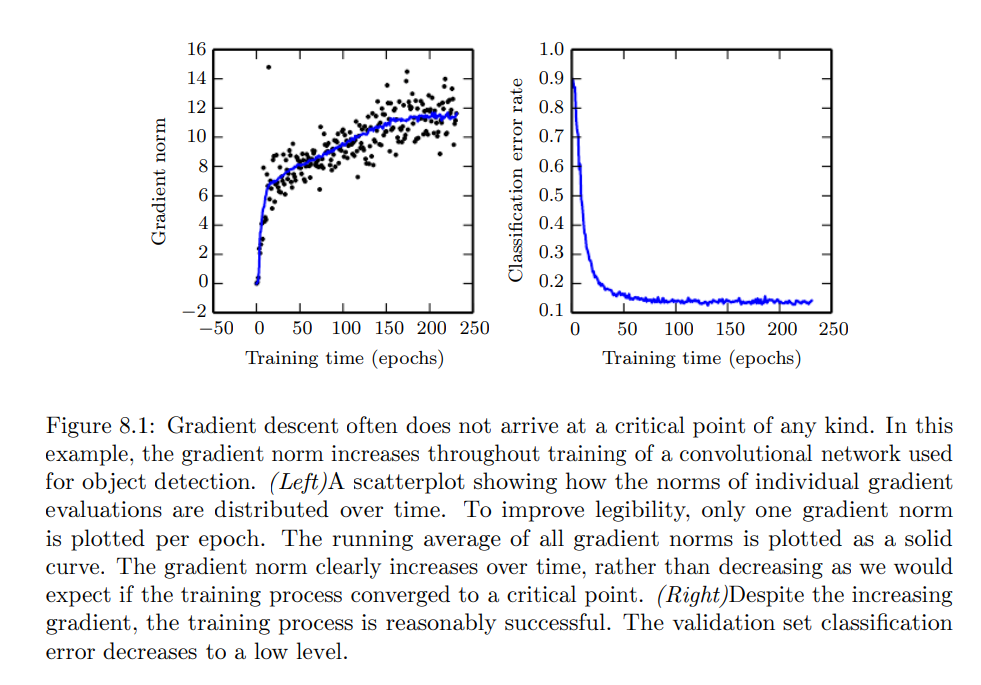
\includegraphics[scale=0.8]{images/Gradient norm.png}
\end{center}

\subsection{Saddle points}
Many classes of random functions exhibit the following behavior: in low dimensional spaces, local minima are common. In higher dimensional spaces, local minima are rare and saddle points are more common. More formally, For a function $f : \mathbb{R}^n \rightarrow \mathbb{R}$ of this type, the expected ratio of the number of saddle points to local minima grows exponentially with $n$. To understand the intuition behind this behavior, observe that the Hessian matrix at a local minimum has only positive eigenvalues. The Hessian matrix at a saddle point has a mixture of positive and negative eigenvalues. In $n$-dimensional space, it is exponentially unlikely that all eigenvalues are positive.\newline\newline
Fortunately, the eigenvalues of the Hessian become more likely to be positive as we reach regions of lower cost. This means that local
minima are much more likely to have low cost than high cost. This happens also for neural networks.\newline\newline
For first-order optimization algorithms that use only gradient information, the gradient can often become very small near a saddle
point. On the other hand, gradient descent empirically seems to be able to escape saddle points in many cases.\newline\newline
For Newton’s method, it is clear that saddle points constitute a problem. Gradient descent is designed to move \textit{downhill} and is not explicitly designed to seek a critical point. Newton’s method, however, is designed to solve for a point where the gradient is zero. Without appropriate modification, it can jump to a saddle point.\newline\newline
There are other kinds of points with zero gradient besides minima and saddle points. There are also maxima, which are much like saddle points from the perspective of optimization—many algorithms are not attracted to them, but unmodified Newton’s method is. Maxima of many classes of random functions become exponentially rare in high dimensional space, just like minima do.\newline\newline
There may also be wide, flat regions of constant value. In these locations, the gradient and also the Hessian are all zero.

\subsection{Cliffs and exploding gradients}
Neural networks with many layers often have extremely steep regions resembling cliffs. On the face of an extremely steep cliff structure, the gradient update step can move the parameters extremely far, usually jumping off of the cliff structure altogether. Fortunately, its most serious consequences can be avoided using the \textbf{gradient clipping} heuristic. The basic idea is to reduce the step size to be small enough that it is less likely to go outside the region
where the gradient indicates the direction of approximately steepest descent.

\subsection{Exploding/Vanishing gradient}
Another difficulty that neural network optimization algorithms must overcome
arises when the computational graph becomes extremely deep. Feedforward
networks with many layers have such deep computational graphs. So do \textbf{recurrent networks}, which construct very deep computational graphs by repeatedly applying the same operation at each time step of a long temporal sequence. Repeated application of the same parameters gives rise to the \textbf{vanishing and exploding gradient problem}. Vanishing gradients make it difficult to know which direction the parameters should move to improve the cost function, while exploding gradients can make learning unstable. The cliff structures described earlier that motivate gradient clipping are an example of the exploding gradient phenomenon.\newline\newline
The vanishing gradient problem can occur also with activation functions that can saturate (e.g. sigmoid) providing gradient close to zero \footnote{basically, weights are no longer updated since the gradient is too small}.\newline\newline
Recurrent networks use the same matrix \textbf{W} at each time step, but feedforward networks do not, so even very deep feedforward networks with non-saturating activation functions (e.g. ReLU) can largely avoid the vanishing and exploding gradient problem.

\subsection{Inexact gradients}
Most optimization algorithms are designed with the assumption that we have
access to the exact gradient or Hessian matrix. In practice, we usually only have a noisy or even biased estimate of these quantities. Nearly every deep learning algorithm relies on sampling-based estimates using a minibatch of training examples to compute the gradient.\newline\newline
In other cases, the objective function we want to minimize is actually intractable. When the objective function is intractable, typically its gradient is intractable as well. In such cases we can only approximate the gradient.\newline\newline
Various neural network optimization algorithms are designed to account for
imperfections in the gradient estimate. One can also avoid the problem by choosing a surrogate loss function that is easier to approximate than the true loss.

\subsection{Local structure not representative of global structure}
Many of the problems we have discussed so far correspond to properties of the loss function at a single point—it can be difficult to make a single step if $J(\theta)$ is poorly conditioned at the current point $\theta$, or if $\theta$ lies on a cliff, or if $\theta$ is a saddle point hiding the opportunity to make progress downhill from the gradient. Optimization based on local downhill moves can fail if the local surface does not point toward the global solution.
\begin{center}
    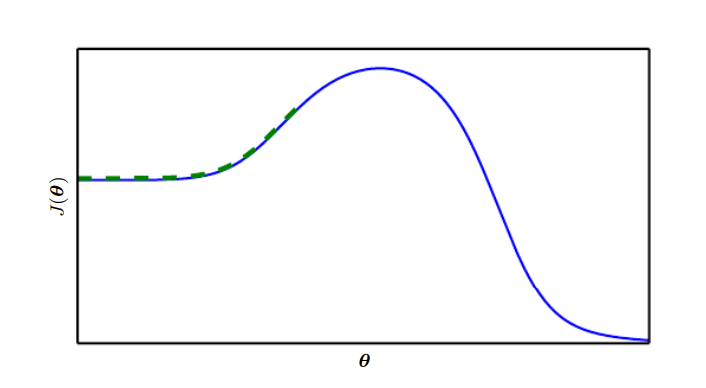
\includegraphics[]{images/bad-init.png}
\end{center}
Much of research into the difficulties of optimization has focused on whether training arrives at a global minimum, a local minimum, or a saddle point, but in practice neural networks do not arrive at a critical point of any kind. The problem in this case is bad initialization.\newline\newline
Many existing research directions are aimed at finding \textbf{good initial points} for problems that have difficult global structure, rather than developing algorithms that use non-local moves. Gradient descent and essentially all learning algorithms that are effective for training neural networks are based on making small, local moves.

\section{Basic Optimization algorithm}
\subsection{Stochastic Gradient Descent}
Stochastic gradient descent (SGD) and its variants are probably the most used optimization algorithms for machine learning in general and for deep learning in particular.
\begin{center}
    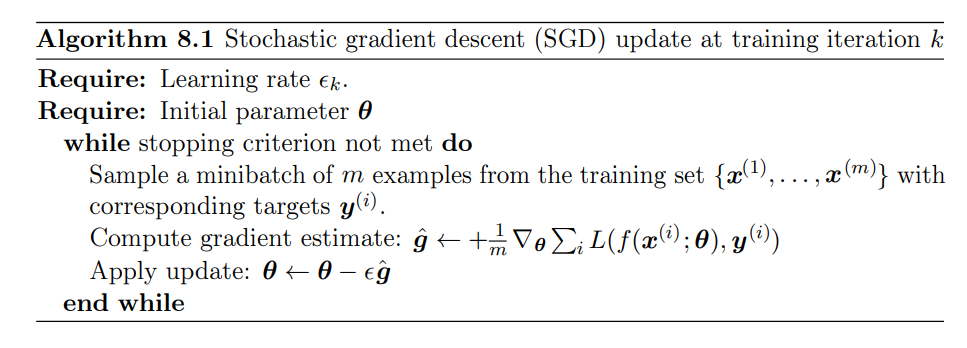
\includegraphics[scale=0.8]{images/SGD.png}
\end{center}
A crucial parameter for the SGD algorithm is the learning rate. In practice, it is necessary to gradually decrease the learning rate over time, so we now denote the learning rate at iteration $k$ as $\epsilon_k$. This is because the SGD gradient estimator introduces a source of noise (the random sampling of m training examples) that does not vanish even when we arrive at a minimum. The true gradient approaches 0 in a minimum, the stochastic estimate doesn’t, so batch gradient descent can use a fixed learning rate. In practice, it is common to decay the learning rate linearly until iteration $\tau$:
\[\epsilon_k = (1 - \alpha)\epsilon_0 + \alpha \epsilon_\tau\]
with $\alpha = \frac{k}{\tau}$. After iteration $\tau$, it is common to leave $\epsilon_\tau$ constant.  
\begin{center}
    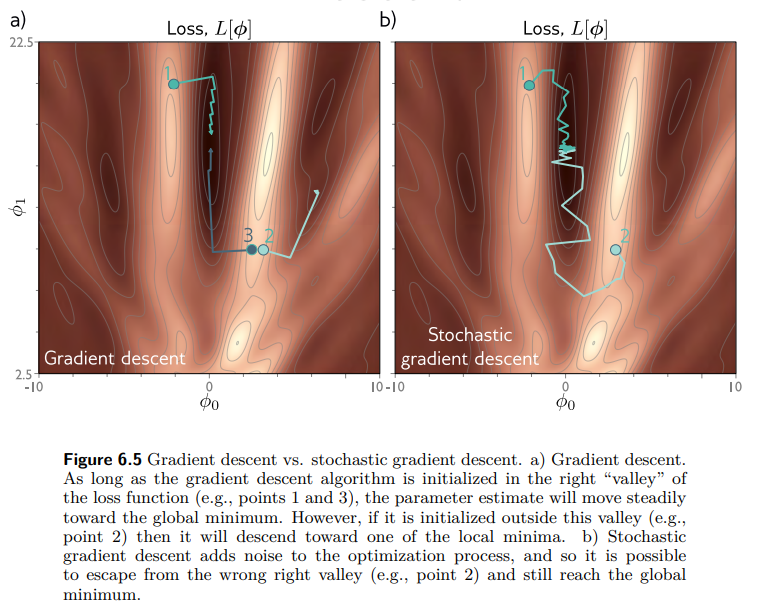
\includegraphics[scale=0.8]{images/SGD vs BGD.png}
\end{center}

\subsection{Momentum}
While stochastic gradient descent remains a very popular optimization strategy, learning with it can sometimes be slow. The method of \textbf{momentum} is designed to accelerate learning, especially in the face of high curvature, small but consistent gradients, or noisy gradients. Furthermore, the problem with gradient descent is that the weight update at a moment ($t$) is governed by the learning rate and gradient at that moment only. It does not take into account the past steps taken while traversing the cost space.
\begin{center}
    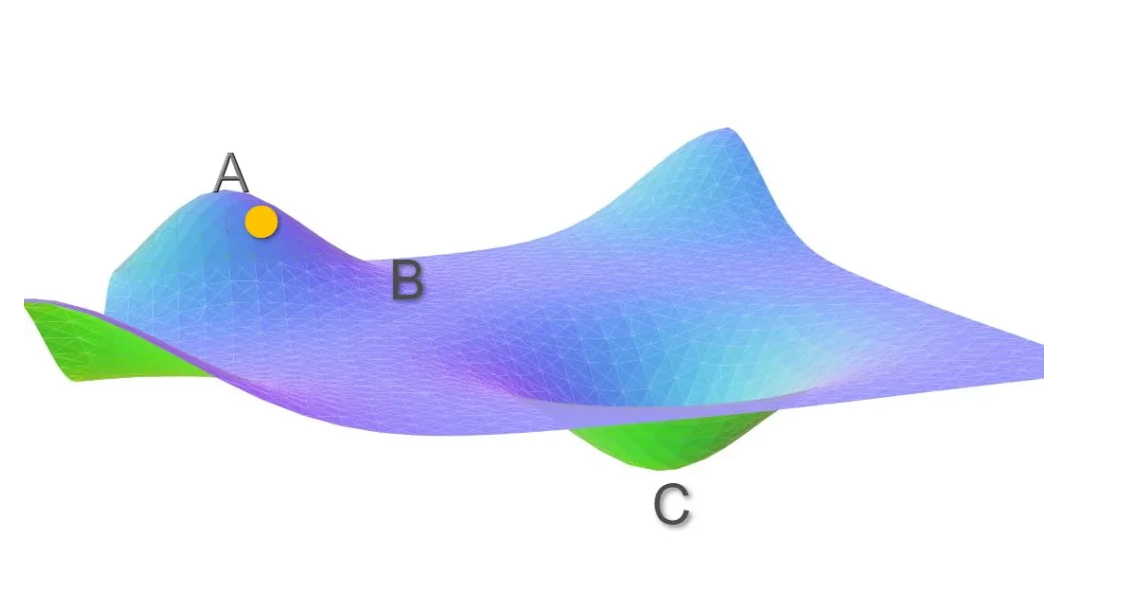
\includegraphics[scale=0.7]{images/momentum.png}
\end{center}
Let’s assume the initial weights of the network under consideration correspond to point A. With gradient descent, the Loss function decreases rapidly along the slope AB as the gradient along this slope is high. But as soon as it reaches point B the gradient becomes very low. The weight updates around B is very small. Even after many iterations, the cost moves very slowly before getting stuck at a point where the gradient eventually becomes zero.\newline\newline
Now, Imagine you have a ball rolling from point A. The ball starts rolling down slowly and gathers some momentum across the slope AB. When the ball reaches point B, it has accumulated enough momentum to push itself across the plateau region B and finally following slope BC to land at the global minima C.\newline\newline
The momentum algorithm accumulates an exponentially decaying moving average of past gradients and continues to move in their direction:
\[\textbf{v}(t) = \alpha\textbf{v}(t - 1) - \epsilon\sigma(t)\]
\[\theta = \theta + \textbf{v(t)}\]
where:
\begin{itemize}
    \item $\textbf{v}(t)$ is called \textbf{velocity} vector and determines the new weight update done at iteration $t$.
    
    \item $\alpha$ is a hyperparameter between 0 and 1 which determines how quickly the contributions of previous gradients exponentially decay.

    \item $\sigma(t) = \nabla_\theta \left(\frac{1}{m}\sum_{i=1}^m L(f(\textbf{x}^{(i)}; \theta), \textbf{y}^{(i)})\right)$ is the gradient at iteration $t$.
\end{itemize}
Assume that $\textbf{v}(0) = 0$:
\begin{equation}
    \begin{split}
        \textbf{v}(0) & = 0 \\
        \textbf{v}(1) & = \alpha\textbf{v}(0) - \epsilon\sigma(1)\\
        \textbf{v}(1) & = -\epsilon\sigma(1) \\
        & \\
        \textbf{v}(2) & = \alpha\textbf{v}(1) - \epsilon\sigma(2)\\
        \textbf{v}(2) & = \alpha (-\epsilon\sigma(1)) -\epsilon\sigma(2)\\
        \textbf{v}(2) & = -\epsilon (\alpha\sigma(1) + \sigma(2))\\
        & \\
        \textbf{v}(3) & = \alpha\textbf{v}(2) - \epsilon\sigma(3)\\
        \textbf{v}(3) & = -\epsilon(\alpha^2\sigma(1) + \alpha\sigma(2) + \sigma(3))
    \end{split}
\end{equation}
Let's \textit{ignore} the learning rate $\epsilon$ and focus on $\alpha$:
\begin{itemize}
    \item with $\alpha = 0.1$, at the third iteration the gradient at $t = 3$ will contribute 100\% of its value, the gradient at $t=2$ will contribute 10\% of its value, and gradient at t=1 will only contribute 1\% of its value (the contribution from earlier gradients decreases rapidly).

    \item with $\alpha = 0.9$, at the third iteration the gradient at $t = 3$ will contribute 100\% of its value, $t=2$ will contribute 90\% of its value, and gradient at $t=1$ will contribute 81\% of its value.
\end{itemize}
From above, we can deduce that the larger $\alpha$, the more previous gradients affect the current direction. Note that the actual contribution of each gradient in the weight update will be further subjected to the learning rate.\newline\newline
Common values of $\alpha$ used in practice include $.5$, $.9$, and $.99$. Like the learning rate, $\alpha$ may also be adapted over time.
\begin{center}
    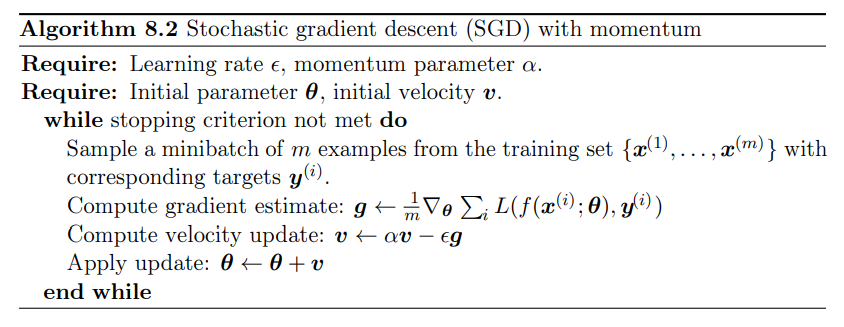
\includegraphics[]{images/Momentum alg.png}
\end{center}
When all the past gradients have the same sign we will take large steps while updating the weights. Even if the learning rate is low, all the gradients along the curve will have the same direction, thus increasing the momentum and accelerating the descent.\newline\newline
Another problem that momentum solves is poor conditioning of the Hessian matrix.
\begin{center}
    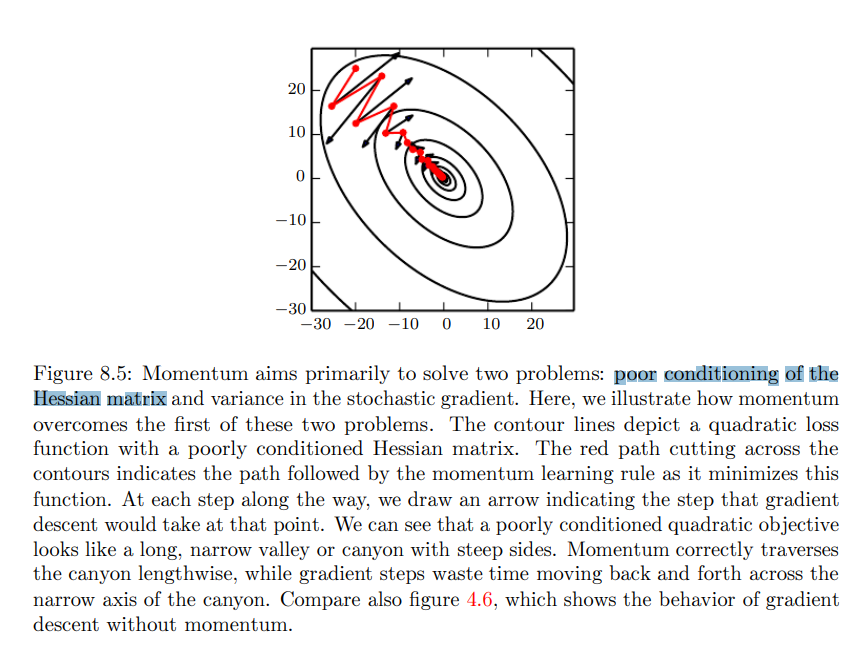
\includegraphics[]{images/poor cond. momentum.png}
\end{center}
In fact, the gradient in one direction is decreased if the gradient direction repeatedly changes as the terms in the sum cancel out.\newline\newline
The overall effect is a smoother trajectory and reduced oscillatory
behavior in valleys
\subsection{Nesterov momentum}
Nesterov momentum introduces a variant of the momentum algorithm. The difference between Nesterov momentum and standard momentum is where the gradient is evaluated. With Nesterov momentum the gradient is evaluated after the current velocity is applied.
\begin{center}
    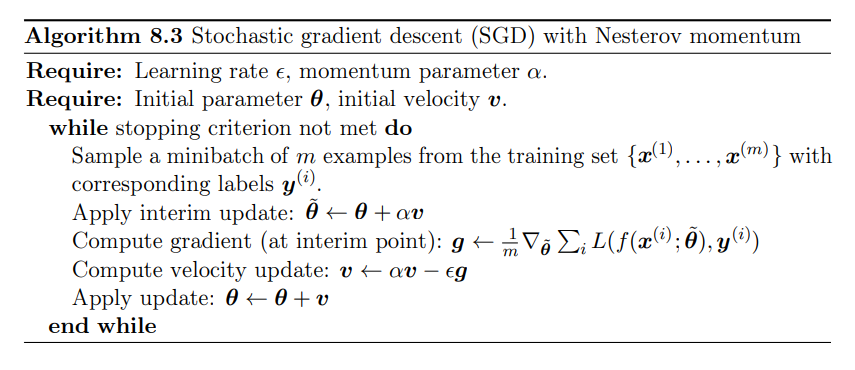
\includegraphics[]{images/nesterov momentum.png}
\end{center}

\section{Parameter initialization}
Deep Learning training algorithms are iterative and depends on initialization. The initial point can determine whether the algorithm converges at all, with some initial points being so unstable that the algorithm encounters numerical difficulties and fails altogether. The use of an optimization algorithm such as stochastic gradient descent that makes small incremental changes to the weights and tends to halt in areas that are nearer to the initial parameters, expresses a
prior that the final parameters should be close to the initial parameters.\newline\newline
Modern initialization strategies are simple and heuristic. Designing improved
initialization strategies is a difficult task because neural network optimization is not yet well understood. Perhaps the only property known with complete certainty is that the initial parameters need to “break symmetry” between different units.\newline\newline
If all the weights in a layer are initialized to the same value, each neuron will compute exactly the same function. The gradient will also be the same, so the weights associated to each neuron will evolve having exactly the same values. In other words, the layer will be equivalent to a layer with only one neuron.\newline\newline
We almost always initialize all the weights in the model to values drawn randomly from a Gaussian or uniform distribution. The choice of Gaussian or uniform distribution does not seem to matter very much, but has not been exhaustively studied. The scale of the initial distribution, however, does have a large effect on both the outcome of the optimization procedure and on the ability of the network to generalize.\newline\newline
Larger initial weights will yield a stronger symmetry breaking effect, helping to avoid redundant units. Initial weights that are
too large may, however, result in exploding values during forward propagation or back-propagation. Large weights may also result in extreme values that cause the activation function to saturate, causing complete loss of gradient through saturated units.\newline\newline
The perspectives of regularization and optimization can give very different insights into how we should initialize a network. The optimization perspective suggests that the weights should be large enough to propagate information successfully, but some regularization concerns encourage making them smaller.\newline\newline
Some heuristics are available for choosing the initial scale of the weights. One heuristic is to initialize the weights of a fully connected layer with $m$ inputs and $n$ outputs by sampling each weight from:
\[U(-\frac{1}{\sqrt{m}}, \frac{1}{\sqrt{m}})\]
while others suggest using the normalized initialization:
\[W_{i,j} \sim U\left( -\sqrt{\frac{6}{m + n}}, \sqrt{\frac{6}{m + n}}   \right)\]
Typically, we set the biases for each unit to heuristically chosen constants, and initialize only the weights randomly.
\subsection{Pre-training}
We can use pre-trained models as starting points for our models. For example:
\begin{itemize}
    \item Unsupervised pre-training: Train an unsupervised model on the training data, use the resulting model as initialization.

    \item Supervised pre-training (transfer learning): Initialize the weights with a model trained on a related task (Especially effective with CNNs).
\end{itemize}

\section{Adaptive learning rates}
Gradient descent with a fixed step size has an undesirable property: it makes:
\begin{itemize}
    \item large adjustments to parameters associated with large gradients (where perhaps we should be more cautious).

    \item small adjustments to parameters associated with small gradients (where perhaps we should explore further).
\end{itemize}
When the gradient of the loss surface is much steeper in one direction than another, it is difficult to choose a learning rate that makes good progress in both directions and is stable. It can make sense to use a separate learning rate for each parameter, and automatically adapt these learning rates throughout the course of learning.
\newline\newline
The delta-bar-delta algorithm is an early heuristic approach
to adapting individual learning rates for model parameters during training. The approach is based on a simple idea: if the partial derivative of the loss, with respect to a given model parameter, remains the same sign, then the learning rate should increase. If the partial derivative with respect to that parameter changes sign, then the learning rate should decrease. Of course, this kind of rule can only be applied to full batch optimization.\newline\newline
More recently, a number of incremental (or mini-batch-based) methods have been introduced that adapt the learning rates of model parameters.

\subsection{AdaGrad}
The AdaGrad algorithm individually adapts the learning rates of all model parameters by scaling them inversely proportional to the square root of the sum of all of the historical squared values of the gradients. Parameters with large partial derivatives will se a rapid decrease in their learning rate.\newline\newline
In the context of convex optimization, the AdaGrad algorithm enjoys some desirable theoretical properties. However, empirically it has been found that—for training deep neural network models—the accumulation of squared gradients from
the beginning of training can result in a premature and excessive decrease in the effective learning rate.
\begin{center}
    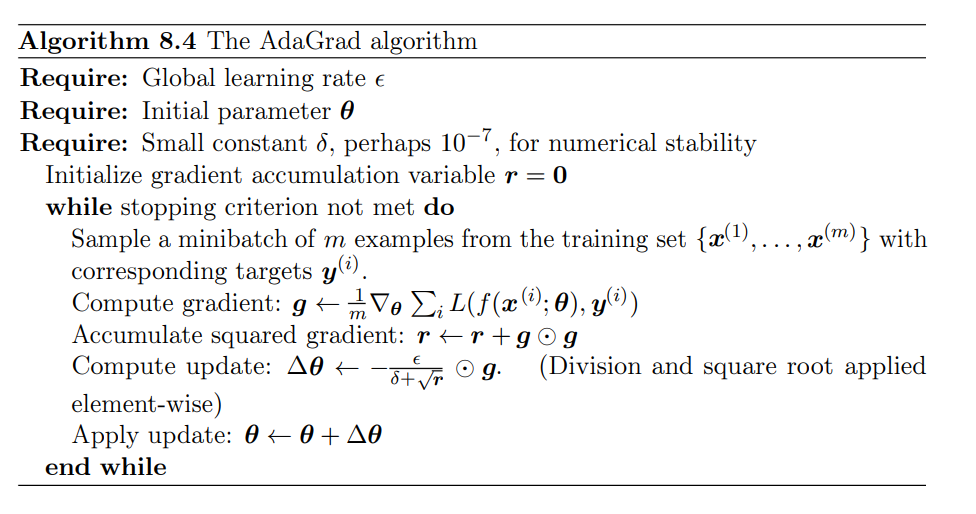
\includegraphics[scale=0.7]{images/AdaGrad.png}
\end{center}

\subsection{RMSprop}
The RMSProp algorithm modifies AdaGrad to perform better in the non-convex setting by changing the gradient accumulation into an exponentially weighted moving average.\newline\newline
Compared to AdaGrad, the use of the moving average introduces a new hyperparameter, $\rho$, that controls the length scale of the moving average. Empirically, RMSProp has been shown to be an effective and practical optimization algorithm for deep neural networks.
\begin{center}
    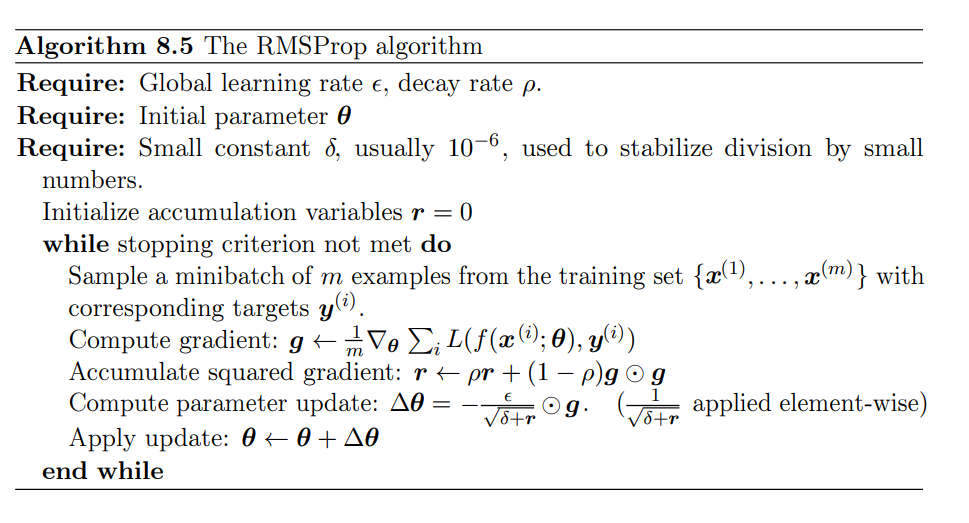
\includegraphics[scale=0.7]{images/RMSProp.png}
\end{center}

\subsection{Adam}
Adam includes bias corrections to the estimates of both the first-order moments (the momentum term) and the (uncentered) second-order moments to account for their initialization at the origin.\newline\newline
Adam is generally regarded as being fairly robust to the choice
of hyperparameters, though the learning rate sometimes needs to be changed from the suggested default.

\section{Second order methods}
In contrast to first-order methods, second-order methods make use of second derivatives to improve optimization. The most widely used second-order method is \textbf{Newton’s method}. Newton’s method is an optimization scheme based on using a second-order Taylor series expansion to approximate $J(\theta)$ near some point $\theta_0$, ignoring derivatives of higher order\footnote{the objective function $J(\theta)$ is the empirical risk}:
\[J(\theta) \approx J(\theta_0) + (\theta - \theta_0)^T \nabla_\theta J(\theta_0) + \frac{1}{2} (\theta - \theta_0)^T \textbf{H}(\theta - \theta_0)\]
where \textbf{H} is the Hessian of $J$ with respect to $\theta$ evaluated at $\theta_0$. If we then solve for the critical point of this function, we obtain the Newton parameter update rule:
\[\theta^* = \theta_0 - \textbf{H}^{-1}\nabla_\theta J(\theta_0)\]
If the function is quadratic, Newton’s method finds directly the minimum, if not, it can be applied iteratively. However, Computing $\textbf{H}$ and $\textbf{H}^{-1}$, is unfeasible for medium-sized networks.\newline\newline
Conjugate gradients is a method to efficiently avoid the calculation of the inverse Hessian by iteratively descending \textbf{conjugate directions}. . The inspiration for this approach follows from a careful study of the weakness of the method of steepest descent, where line searches are applied iteratively in the direction associated with the gradient.\newline\newline
In the method of conjugate gradients, we seek to find a search direction that is conjugate to the previous line search direction, i.e. it will not undo progress made in that direction. At training iteration $t$, the next search direction $\textbf{d}_t$ takes the form:
\[\textbf{d}_t = \nabla_\theta J(\theta) + \beta_t \textbf{d}_{t-1}\]
where $\beta_t$ is a coefficient whose magnitude controls how much of the direction, $\textbf{d}_{t-1}$, we should add back to the current search direction.\newline\newline
Two directions, $\textbf{d}_t$ and $\textbf{d}_{t-1}$, are defined as conjugate if $\textbf{d}_t^T \textbf{H}\textbf{d}_{t-1} = 0$, where $\textbf{H}$ is the Hessian matrix. Fortunately, we can compute the correct $\beta_t$ without computing $\textbf{H}$.\newline\newline
For quadratic surfaces in $k$ dimensions, conjugate gradients method requires at most $k$ steps to achieve the minimum (it can be adapted for non-quadratic surfaces).


\section{Batch normalization}
LeCun et al. (1998) showed that normalizing the inputs speeds
up training. Loffe and Szegedy (2015) proposed Batch Normalization to normalize hidden (pre-)activations:
\begin{itemize}
    \item each unit’s pre-activation is normalized (mean subtraction, standard deviation division).

    \item during training, mean and standard deviation is computed for each mini-batch.

    \item backpropagation takes into account the normalization.

    \item at test time, the global mean and global standard deviation is used. It requires a final phase where, from the first to the last hidden layer:
    \begin{itemize}
        \item propagate all training data to that layer.
        \item compute and store the global mean and global standard deviation for each unit.
    \end{itemize}

\end{itemize}
Normalize the pre-activation can help to keep the pre-activation in a non-saturating regime. 

